\chapter{Bramka fazowa bazująca na fazie geometrycznej}
\label{chap:phaseGate}

\section*{Opis rozdziału}

W tym rozdziale zostały opisane wyniki przedstawione w pracy~\cite{wieckowski.mierzejewski.2020}.
W pracy badano dynamikę pojedynczego qubitu zakodowanego na czterech \MZM.
Zostanie tutaj pokazane, że wyplatanie częściowo przekrywających \MZM, można wykorzystać do implementacji bramki fazowej bazującej na fazie geometrycznej.

\section{Pojedyncze wyplatanie i testy adiabatyczności}

Fundamentalnym problemem dla komputerów kwantowych jest implementacja zestawu bramek, który gwarantowałby uniwersalność obliczeń.
Przykładem takiego zestawu jest zbiór zawierający: bramkę Hadamarda $\hadamard$, bramkę fazową $\phaseGate$ oraz bramkę $\CNOT$~\cite{nielsen.chuang.2011}.
Bramkę $\hadamard$ oraz $\CNOT$ można zrealizować z wykorzystaniem \MZM\ z zagwarantowaną ochroną topologiczną (patrz rozdział~\ref{chap:topologicalQuantumComputing}).
Problematyczna jest bramka $\phaseGate$.
Operacje grupy warkoczowej $\braidGroup$, do której należą \MZM, nie są wystarczające do implementacji bramki $\phaseGate$.
Rozwiązanie, które omija ten problem, polega na zbliżeniu do siebie \MZM\ ~\cite{sarma.freedman.2015}. Przekrywanie \MZM, na skutek ich zbliżenia, powoduję zniesienie degeneracji $\deltaE$ (patrz sekcja~\ref{sec:universalQuantumComputing}) co prowadzi do przesunięcia fazy.
To przesunięcie związane jest z fazą dynamiczną, ponieważ przy zniesionej degeneracji $\deltaE\neq0$ (patrz sekcja~\ref{sec:universalQuantumComputing}).
W rezultacie zmiana fazy qubitu, zależna jest od $\deltaE$ oraz czasu $\Delta\timeNormal$ trwania takiej operacji zbliżania i oddalania \MZM.
Należy tutaj podkreślić, że taka operacja nie jest chroniona żadną symetrią i w konsekwencji musi zostać przeprowadzona odpowiednia korekcja błędów, np. z wykorzystaniem \textit{destylacji magicznych stanów} ~\cite{bravyi.kitaev.2005,sarma.freedman.2015}.
Z~taką bramką fazową związana jest faza dynamiczna $\phaseGatei\PhiDyn$.
Taka bramka jest kontrolowana przez dwa parametry: degenerację $\deltaE$ oraz czas trwania $\Delta\timeNormal$.
W tym rozdziale przedstawiono inne podejście do konstrukcji $\phaseGate$ dla qubitu bazującego na \MZM.
Procedura ta polega na podwójnym wyplataniu \MZM, które częściowo się przekrywają.
Po wyplataniu \MZM, które się przekrywają, faza geometryczna $\PhiGeo$, odbiega od wartości tej fazy dla przypadku, kiedy \MZM\ są całkowicie odseparowane~\cite{sekania.plugge.2017}.
Niestety, przy przekrywających się \MZM, w układzie pojawia się niezerowa degeneracja $\deltaE$ co prowadzi do pojawienia się dodatkowej fazy dynamicznej $\PhiDyn$.
W pracy ~\cite{wieckowski.mierzejewski.2020} pokazaliśmy, że fazę dynamiczną $\PhiDyn$ można wyeliminować, kiedy układ ma symetrię cząstka--dziura.

\begin{figure}
\centering
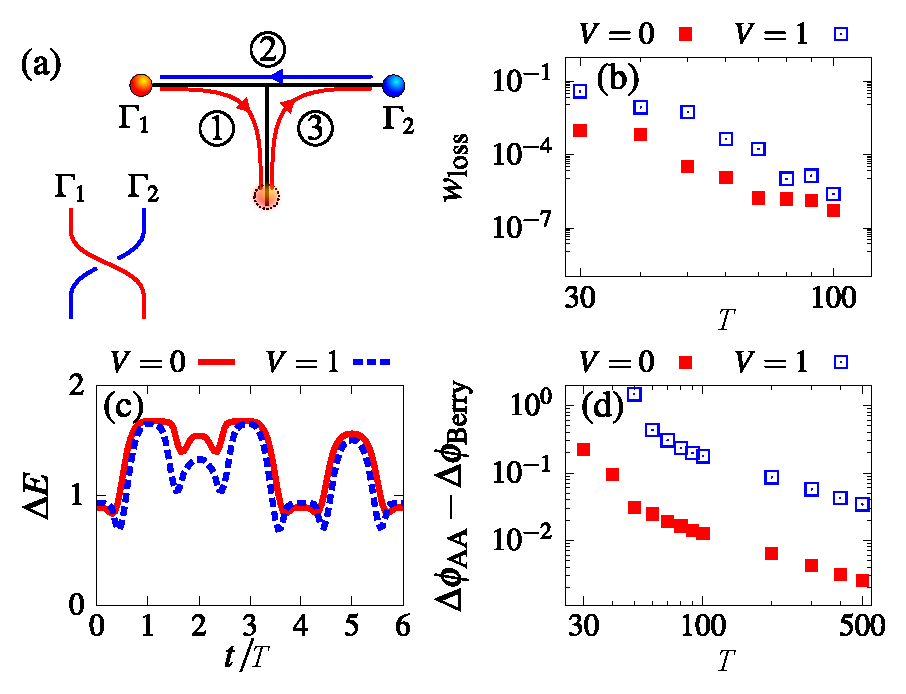
\includegraphics[width=0.8\textwidth]{04-Includes/Figures/PhaseGate/fig1.pdf}
\caption
[Test adiabatyczności wymiany \textit{MZM}.]
{
(a) Schematyczne trójzłącze z \MZM\ $\Gammaii_1$, $\Gammaii_2$. 
Strzałkami zaznaczono proces wyplatania quasicząstek.
(b) Straty wiarygodności $\fidelity$ w funkcji całkowitego czasu ewolucji  $\timeTotal=6\timePartial$.
(c) Szczelina energetyczna w funkcji $\timeNormal/\timePartial$.
(d) Różnica $\Delta\PhiAA-\Delta\PhiBerry$ w funkcji $\timePartial$.
Wyniki dla $\sites=7$, $\DeltaSCuniform=0.5$ oraz $\muuniform=0$.
}
\label{fig:phaseGate1}
\end{figure}

\begin{figure}
\centering
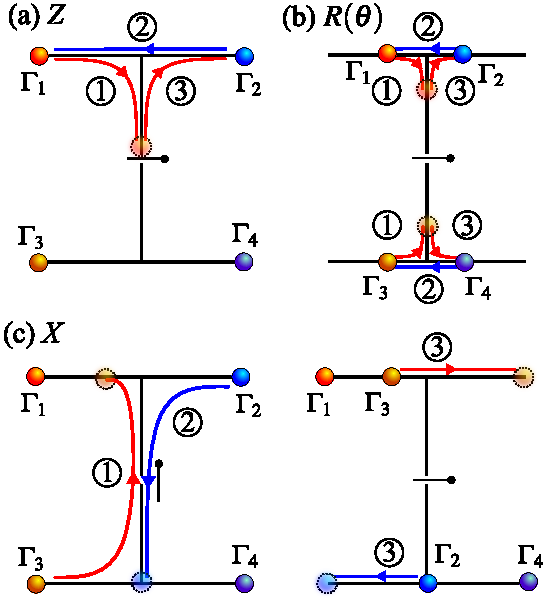
\includegraphics[width=0.6\textwidth]{04-Includes/Figures/PhaseGate/fig2.pdf}
\caption
[Układ dwóch trójzłącz wraz z realizacją wybranych bramek kwantowych.]
{
Układ dwóch trójzłącz zwierających \MZM, $\Gammaii_1$, $\Gammaii_2$, $\Gammaii_3$, $\Gammaii_4$ , wraz z realizacją wybranych bramek kwantowych.
Podwójna realizacja przedstawionych kroków wyplatania jest równoważna
(a) bramce $\zgate$;
(b)~bramce fazowej $\phaseGate$;
(c) bramce $\xgate$.
}
\label{fig:phaseGate2}
\end{figure}

Podobnie jak w sekcji~\ref{sec:quantumGates},
rozważono qubit zakodowany na dwóch parach \MZM: $\Gammaii_1$, $\Gammaii_2$, $\Gammaii_3$, $\Gammaii_4$, gdzie para $\Gammaii_1$, $\Gammaii_2$ związana jest ze złączem $\trijunction{12}$, a para $\Gammaii_3$, $\Gammaii_4$ ze złączem $\trijunction{34}$.
Każda para \MZM\ umieszczona była na pojedynczym trójzłączu. Trójzłącze $\trijunction{12}$ zostało schematycznie przedstawione na rysunku~\ref{fig:phaseGate1}(a).
Cały układ dwóch połączonych trójzłącz został przedstawiony na rysunku~\ref{fig:phaseGate2}.
Baza qubitu zawiera dwa stany oba należące do podprzestrzeni z~parzystą liczbą cząstek [patrz równanie~\labelcref{eq:state0,eq:state1}]:
\begin{align}
    \qstate{0} &= \eeven= \qstate{e_{12}}\,\kron\, \qstate{e_{34}},\label{eq:braidQubitBase1}\\
    \qstate1 &= \oodd = \qstate{o_{12}}\,\kron\, \qstate{o_{34}}.\label{eq:braidQubitBase2}
\end{align}
Stany $\qstate{o_{12}}$, $\qstate{o_{34}}$ są związane odpowiednio ze złączem $\trijunction{12}$ oraz $\trijunction{34}$ (analogicznie stany z parzystą liczbą cząstek).
Zbadano minimalny układ, który umożliwia wyplatanie \MZM\ --- trójzłącze~\cite{alicea.oreg.2011,sekania.plugge.2017}.
Rozważono trzy łańcuchy równej długości $\sitesChain$, każdy z inną fazą nadprzewodzącego parametru porządku $\DeltaSC=\DeltaSCuniform \exp(-\iu \PhiSC)$, gdzie $\PhiSC=0,\,+\frac{\pi}2,\,-\frac{\pi}2$ odpowiednio w lewym, prawym i pionowym łańcuchu [patrz rysunek~\ref{fig:phaseGate1}(a)].
Założono, że każde złącze zawiera $\sites=3\sitesChain+1$ węzłów i jest opisane hamiltonianem modelu Kitaeva \eqref{eq:kitaev+V}
\begin{equation}
    \hatH_{\text{Kitaev}+V}^{\text{trijunction}}(\timeNormal) = 
    \sum_{\langle i,j\rangle}\left[
    \left(\tuniform \, \aid \aj + \DeltaSC\, \aid \ajd\right)
    + \hc + \Vuniform \nz{i} \nz{j}\right] + 
    \sum_{i=1}^{\sites} \mui(\timeNormal) \nz{i}.\label{eq:kitaev+braiding}
\end{equation}
W obliczeniach przyjęto bezwymiarowe jednostki $\HBAR=\tuniform=1$.
Główną motywacją badania układu z oddziaływaniami wielociałowymi $\Vuniform$, przy procesie wyplatania \MZM, jest fakt, że w~przypadku (quasi-)jednowymiarowych układów, nawet słabe oddziaływanie kulombowskie potrafi znacząco wpłynąć na własności materiałów.
W przypadku braku nadprzewodzącego parametru porządku, $\DeltaSCuniform=0$, nanodruty mogą być opisane jako oddziałujące ciecze Luttigera~\cite{haldane.1981}.
\MZM\ nie są całkowicie odporne na oddziaływania wielociałowe~\cite{gangadharaiah.braunecker.2011,manolescu.marinescu.2014,thomale.rachel.2013,wieckowski.maska.2018,wieckowski.ptok.2019,peng.pientka.2015,ng.2015,chan.chiu.2015,hofmann.assaad.2016}, a~niezbyt silne oddziaływania mogą nawet je stabilizować~\cite{dominguez.cayao.2017,stoudenmire.alicea.2011,gergs.fritz.2016,hassler.schuricht.2012}.

W celu przesuwania \MZM\ w obrębie łańcuchów można odpowiednio manipulować potencjałem chemicznym $\mui$, na poszczególnych węzłach odpowiednio zmieniając wielkość obszaru topologicznego poprzez przesuwanie granic tego obszaru.
Tak jak napisano w sekcji~\ref{sec:kitaev}, kiedy $|\DeltaSCuniform|>0$ w modelu Kitaeva (bez oddziaływań) występują dwie fazy~\cite{kitaev.2001}: topologiczna dla $|\muuniform| \le 2\tuniform$ oraz trywialna dla $|\muuniform| > 2\tuniform$.
Wyplatanie dokonywane jest poprzez adiabatyczną ewolucję $\mui(\timeNormal)$ w taki sposób, że część węzłów pozostaje w fazie trywialnej, pozostałe w fazie topologicznej~\cite{alicea.oreg.2011}.
Wykorzystano identyczny protokół do zmiany $\mui(\timeNormal)$ jak w pracy~\cite{sekania.plugge.2017}. 
Potencjał zmieniano w następujący sposób
\begin{equation}
    \mui(\timeNormal) = \muuniform_c g_i(\timeNormal) + \muuniform,\label{eq:muprotocol}
\end{equation}
gdzie $\muuniform$ to jednorodny potencjał chemiczny,  $\muuniform_c=\pm4$, $g_i(\timeNormal)\in[0,1]$.
Wartości $\muuniform_c$ wybrano odpowiednio duże, żeby mieć gwarancję, że węzły dla których $\mui=\muuniform_c$ były w fazie trywialnej nawet dla układu z oddziaływaniami. 
Funkcja $g_i(\timeNormal)$ to gładka funkcja dana wzorem
\begin{equation}
    g_i(\timeNormal) = m\left\{\frac{\timeNormal}{\timePartial}\left[1+\kappa(\sitesChain-1)\right] -\kappa(\sitesChain-i)\right\}, \qquad \timeNormal\in[0,\timePartial]
\end{equation}
gdzie $\timePartial$ to czas trwania pojedynczej sekwencji zmieniania potencjału $\mui(\timeNormal)$ na wybranym łańcuchu złącza (więcej patrz kolejny akapit). Parametr $\kappa=0.025$, a $m(x)$ to skalarna funkcja
\begin{equation}
    m(x) = \sin^2\left[\tfrac{\pi}2 r(x) \right], \quad r(x) = \min[\max(x,0),1].
\end{equation}
Funkcja $g_i(\timeNormal)$ opisuje w jaki sposób potencjał $\mui(\timeNormal)$ rośnie w czasie na poszczególnych węzłach.
Dla procesu odwrotnego, t.j. kiedy $\mui(\timeNormal)$ malał, zmieniano $\timeNormal\to\timePartial-\timeNormal$.

Następnie rozważono pojedyncze wyplatanie dwóch \MZM, na pojedynczym trójzłączu $\trijunction{12}$ [rysunek~\ref{fig:phaseGate1}(a) oraz~\ref{fig:phaseGate2}(a)].
Jako warunek początkowy, na węzłach pionowego łańcucha ustawiono $\mui(0)=\muuniform_c$ (faza trywialna), a na węzłach pozostałych poziomych łańcuchów $\mui(0)=0$ (faza topologiczna).
Na każdym krańcu łańcuchów poziomych, lewego i prawego, mogą znajdować się odpowiednio $\Gammaii_1$ oraz $\Gammaii_2$.
W kolejnych krokach, korzystając z równania~\eqref{eq:muprotocol}, 
odpowiednio manipulując potencjałami $\mui(\timeNormal)$ wymieniano miejscami $\Gammaii_1$, $\Gammaii_2$ [rysunek~\ref{fig:phaseGate1}(a)].
Procedura wyplatania została podzielona na 6 segmentów, każdy trwający czas $\timePartial$:
\begin{enumerate}
\item[(\textit{i})] $\timeNormal\in(0,\timePartial)$
przemieszczanie $\Gammaii_1$ na środek trójzłącza;

\item[(\textit{ii})] $\timeNormal\in(\timePartial,2\timePartial)$
przemieszczanie $\Gammaii_1$ na koniec pionowego łańcucha;

\item[(\textit{iii})] $\timeNormal\in(2\timePartial,3\timePartial)$
przemieszczanie $\Gammaii_2$ na środek trójzłącza;

\item[(\textit{iv})] $\timeNormal\in(3\timePartial,4\timePartial)$
przemieszczanie $\Gammaii_2$ na koniec lewego łańcucha;

\item[(\textit{v})] $\timeNormal\in(4\timePartial,5\timePartial)$
przemieszczanie $\Gammaii_1$ na środek trójzłącza;

\item[(\textit{vi})] $\timeNormal\in(5\timePartial,6\timePartial)$
przemieszczanie $\Gammaii_1$ na koniec prawego łańcucha.

\end{enumerate}
Na rysunku~\ref{fig:phaseGate3} przedstawiono schematycznie poszczególne wymienione wyżej kroki wyplatania $\Gammaii_1$ oraz $\Gammaii_2$.
Szczegółowe przebiegi funkcji $\mui(\timeNormal)$ zostały przedstawione na rysunku~\ref{fig:phaseGate4}.

\begin{figure}
\centering
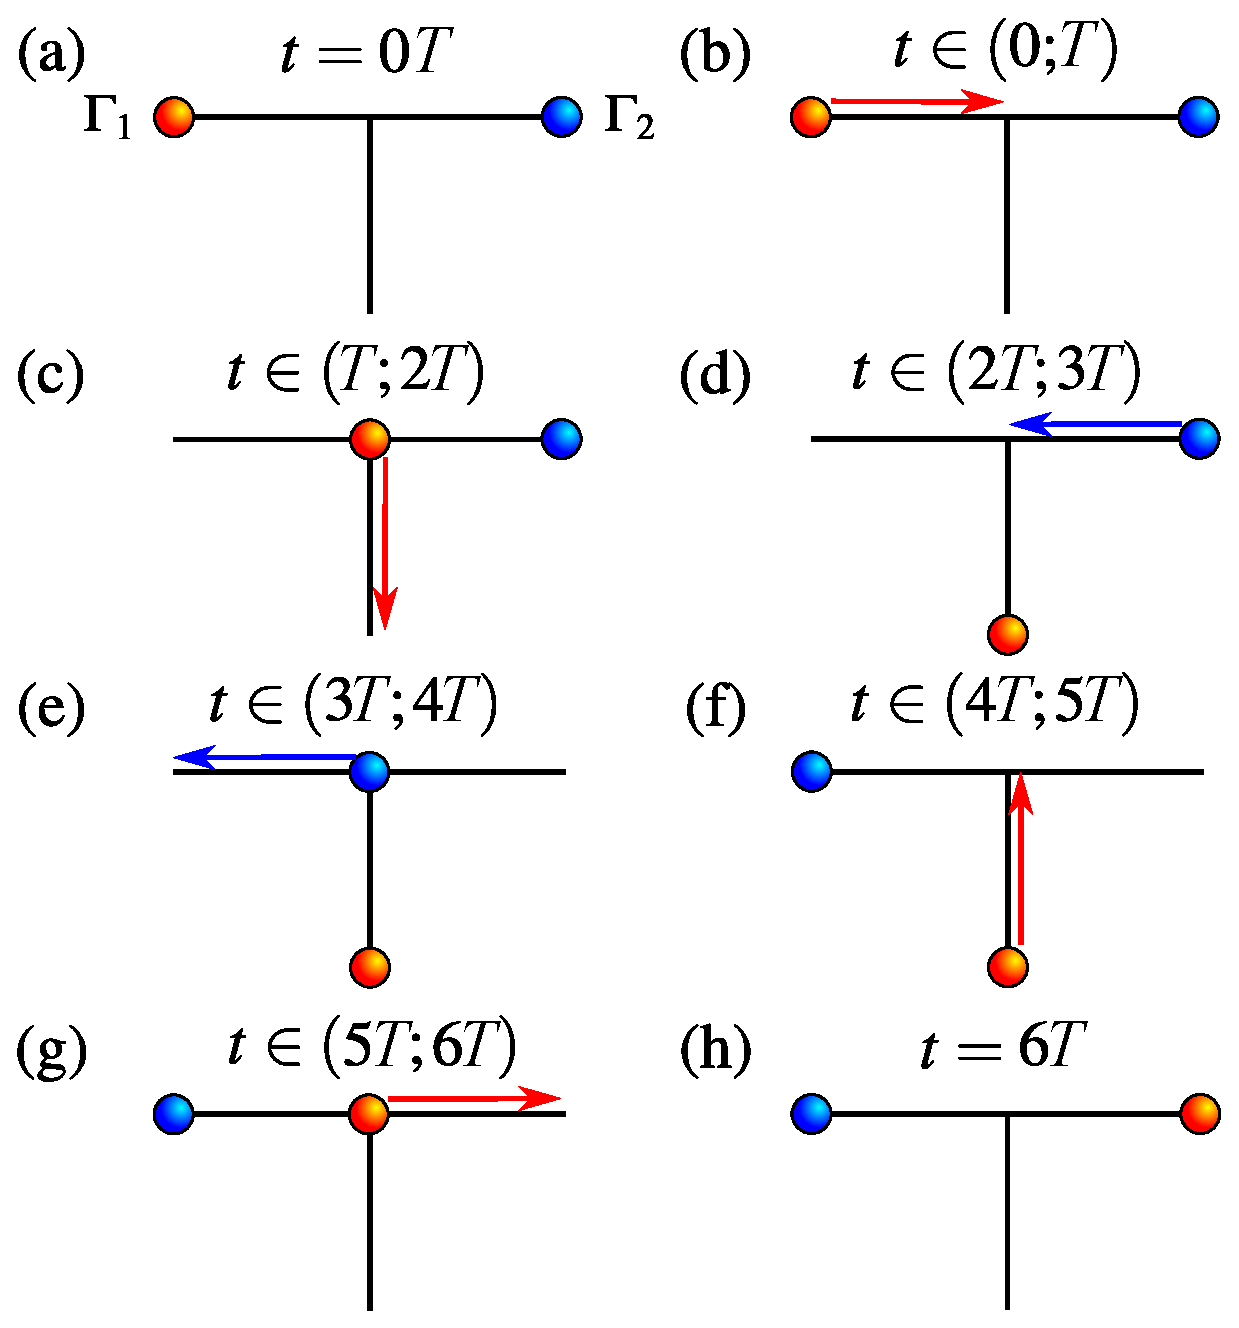
\includegraphics[width=0.6\textwidth]{04-Includes/Figures/PhaseGate/fig8.pdf}
\caption
[Schematyczny protokół wyplatania \textit{MZM} na trójzłączu]
{Schematyczny protokół wyplatania $\Gammaii_1$ oraz $\Gammaii_2$ na złączu $\trijunction{12}$.}
\label{fig:phaseGate3}
\end{figure}

\begin{figure}
\centering
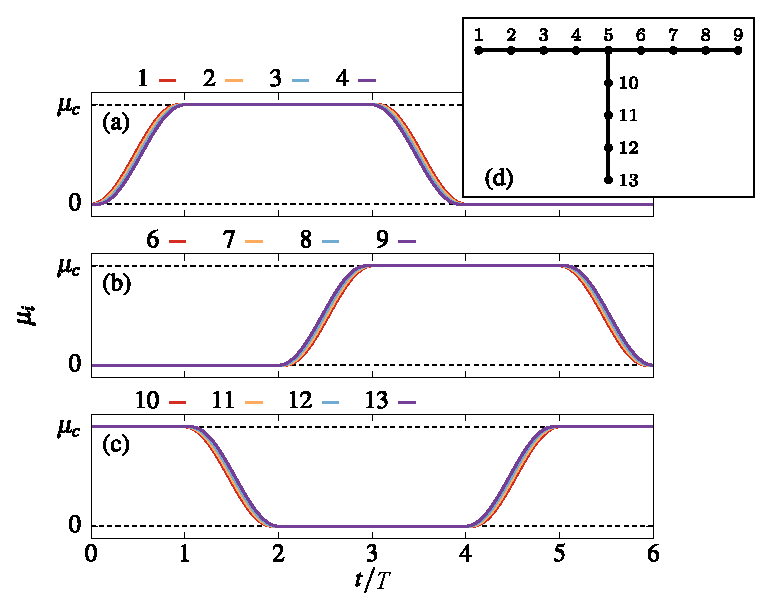
\includegraphics[width=0.8\textwidth]{04-Includes/Figures/PhaseGate/fig9.pdf}
\caption
[Standardowy protokół wyplatania -- potencjał $\mu_i$ w funkcji $t/T$.]
{
Standardowy protokół wyplatania --  potencjał $\mui$ w funkcji $\timeNormal/\timePartial$ dla
(a)~lewego;
(b)~prawego;
(c)~pionowego łańcucha trójzłącza.
(d)~Numeracja węzłów. Przykład dla układu o $\sites=13$.
}
\label{fig:phaseGate4}
\end{figure}

Zmiany parametru $\mui(\timeNormal)$ przedstawione w poprzednim akapicie opisują cykliczną ewolucję hamiltonianu~\eqref{eq:kitaev+braiding}.
W celu badania pełnej dynamiki kwantowej rozwiązywano równanie Schr\"odingera (\acrshort{TDSE}) [patrz równanie~\eqref{eq:timeDependentSchrodingerEquation}].
Jako warunek początkowy $\qstate {\psi(0)}$ przyjęto stan podstawowy początkowego hamiltonianu $\hatH(0)$ [równanie~\eqref{eq:kitaev+braiding}].
Równanie Sch\"odingera rozwiązywano z wykorzystaniem schematu bazującego na wielomianach Czebyszewa, który został opisany w rozdziale~\ref{chap:dynamics}.
Przyjęto krok $\delta t=0.01$ oraz w rozwinięciu w szereg wielomianów Czebyszewa skorzystano z $M=10$ pierwszych wyrazów.
W pierwszym kroku zbadano cykliczność oraz adiabatyczność ewolucji wyplatania ~[patrz sekcja~\ref{sec:phaseFactors}].
Aby ewolucja była cykliczna, straty wiarygodności powinny dążyć do zera $\fidelity\to0$.
Takie zachowanie jest wyraźnie widoczne w zaprezentowanych wynikach na rysunku~\ref{fig:phaseGate1}(b).
Dla czasów $\timePartial>100$ straty wiarygodności stają się pomijalne.
Warunkiem koniecznym ewolucji adiabatycznej jest to, że szczelina energetyczna $\DeltaE$ pomiędzy stanem podstawowym, a wzbudzonym powinna być większa od zera na całej ścieżce ewolucji.
Należy tutaj przypomnieć, że układ opisany modelem Kitaeva, jest chroniony symetrią parzystości i przejścia pomiędzy stanami z dwóch różnych podprzestrzeni parzystości są niedozwolone.
Jako kryterium szczeliny energetycznej przyjęliśmy minimalną szczelinę z dwóch podprzestrzeni
\begin{equation}
    \DeltaE = \min(\Energy_1^e-\Energy_0^e,\Energy_1^o-\Energy_0^o),
\end{equation}
gdzie $\Energy_n^{e(o)}$ to $n$-ta energia własna odpowiednio z podprzestrzeni z parzystą (nieparzystą) liczbą cząstek.
Wyniki dla $\DeltaE$ zostały przedstawione na rysunku~\ref{fig:phaseGate1}(c).
Szczelina nie zamyka się, nawet w przypadku układu z oddziaływaniami wielociałowymi. 
Przy dostatecznie dużym czasie $\timePartial$, ewolucja powinna być traktowana jak ewolucja adiabatyczna.
Jako ostateczny test adiabatyczności ewolucji porównano fazę Aharonova--Anandana $\PhiAA$ z fazą Berry'ego $\PhiBerry$.
Na rysunku~\ref{fig:phaseGate1}(d) przestawiono różnicę $\DeltaPhiAA-\DeltaPhiBerry$ w funkcji czasu $\timePartial$.
Wydaje się, że ta różnica dla $\timePartial\to\infty$ dąży do zera, nawet dla układu o niezerowych oddziaływaniach wielociałowych, co potwierdza słuszność stosowania przybliżenia adiabatycznego.
W dalszych rozważaniach skupiono się tylko i wyłącznie na ewolucji adiabatycznej.

\begin{figure}
\centering
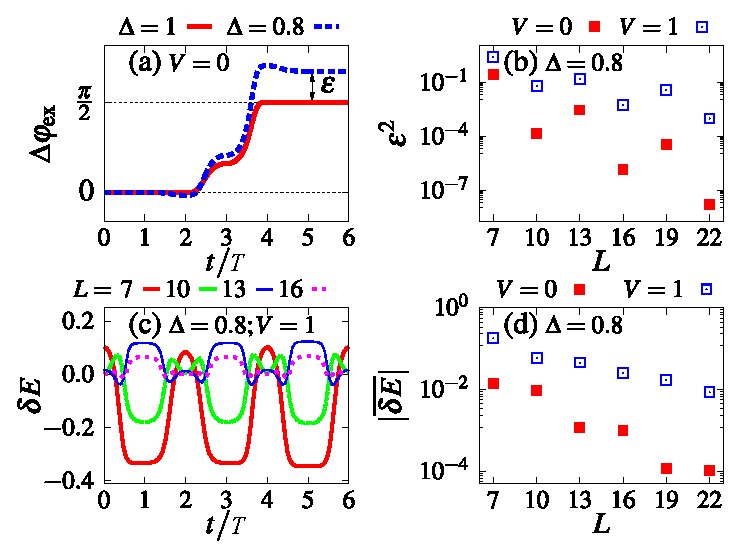
\includegraphics[width=0.8\textwidth]{04-Includes/Figures/PhaseGate/fig3.pdf}
\caption
[Pojedyncza operacja wyplatania na pojedynczym trójzłączu.]
{Pojedyncza operacja wyplatania na pojedynczym trójzłączu.
Wyniki dla $\muuniform=0$.
(a) Faza wymiany $\DeltaPhiEx$ w funkcji czasu $\timeNormal/\timePartial$ ($\sites=7$);
(b)~\acrshort{FSS} błędu wyplatania $\braidingError$;
(c)~degeneracja stanu podstawowego $\deltaE$;
(d)~\acrshort{FSS} uśrednionej degeneracji stanu podstawowego $|\deltaE|$.
}
\label{fig:phaseGate5}
\end{figure}


Na rysunku~\ref{fig:phaseGate5}(a) przedstawiono różnicę fazy wymiany $\DeltaPhiEx$ [równanie~\eqref{eq:exchangePhaseDef}] pomiędzy poszczególnymi podprzestrzeniami parzystości.
Warto tutaj jeszcze raz podkreślić, że faza wymiany $\DeltaPhiEx$ nie jest niezmiennikiem cechowania i może zależeć od poszczególnych realizacji protokołu.
Faza wymiany może stanowić cenną wskazówkę podczas analizy danej realizacji protokołu.
Ta faza była analogicznie stosowana m.in. w następujących pracach~\cite{cheng.he.2016,sekania.plugge.2017,ezawa.2019}.
Dla $\DeltaSCuniform=1$, w przypadku bez oddziaływań wielociałowych, \MZM\ są zlokalizowane na pojedynczych węzłach sieci, są przestrzennie rozseparowane i nie przekrywają się nawet dla układów o skończonej liczbie węzłów.
Dla takiego przypadku $\DeltaPhiBerry=\frac{\pi}{2}$, co perfekcyjnie zgadza się z przedstawionym wynikiem na rysunku~\ref{fig:phaseGate5}(a) [patrz $\DeltaPhiEx$ na końcu ewolucji dla $\timeNormal=6\timePartial$].
W przypadku kiedy $\DeltaSCuniform\neq1$, \MZM\ przekrywają się, a otrzymana faza $\DeltaPhiBerry$  jest odchylona od wartości $\frac{\pi}2$ o pewien błąd wyplatania $\braidingError=\DeltaPhiBerry-\frac{\pi}{2}$.
Ten błąd $\braidingError$  jest efektem skończonego rozmiaru, co zostało rozpoznane w skalowaniu rozmiarowym (\acrshort{FSS}) na  rysunku~\ref{fig:phaseGate5}(b).
W przypadku nieskończonego układu $\sites\to\infty$, kiedy \MZM\ są całkowicie rozseparowane, wydaje się, że błąd wyplatania $\braidingError$ zanika do zera.

Z przekrywaniem \MZM\ na skończonym układzie, związane jest pewne rozszczepienie energetyczne $\deltaE$ związane ze zniesieniem degeneracji stanu podstawowego.
Brak perfekcyjnej degeneracji $\deltaE\neq0$ powoduje pojawienie się w układzie fazy dynamicznej $\DeltaPhiDyn\neq0$.
Na rysunku~\ref{fig:phaseGate5}(c) przedstawiono, jak rozszczepienie $\deltaE$ zmienia się w czasie ewolucji $\timeNormal/\timePartial$ dla różnych rozmiarów układu.
Wraz ze wzrostem rozmiaru układu $\deltaE$ maleje.
W celu dokładniejszego przedyskutowania rozszczepienia $\deltaE$, 
policzono uśrednione rozszczepienie po całej ewolucji, korzystając z następującego wzoru
\begin{equation}
    \widebar{\deltaE} = \frac{1}{\timeTotal}\int\limits_0^{\timeTotal}\text d\timeNormal\, \deltaE(\timeNormal),
\end{equation}
gdzie $\timeTotal$ to całkowity czas ewolucji (w przypadku pojedynczej operacji wyplatania $\timeTotal=6\timePartial$).
Taka uśredniona wielkość $\widebar \deltaE$ związana jest bezpośrednio z różnicą faz dynamicznych $\DeltaPhiDyn=\timeTotal\widebar\deltaE$.
Na rysunku~\ref{fig:phaseGate5}(d) przedstawiono skalowanie rozmiarowe uśrednionego rozszczepienia energii $\widebar{\deltaE}$.
Zarówno dla układu z oddziaływaniami jak i bez oddziaływań wielociałowych, $\widebar{\deltaE}$ zanika niemal wykładniczo wraz z rosnącym rozmiarem układu $\sites$.

Niezerową wartość błędu wyplatania $\braidingError$ można wykorzystać do realizacji bramki fazowej bazującej na fazie geometrycznej.
Równocześnie przy niezerowej wartości $\braidingError$ w układzie pojawia się niezerowa faza dynamiczna, co nie jest korzystne dla implementacji bramki fazowej.
Problem fazy dynamicznej udało się rozwiązać, co zostanie przedstawione w kolejnej sekcji.

\ornament

\section{Realizacja bramki fazowej}\label{sec:phaseGateRealization}

W celu pokazania, że fazę dynamiczną można wyeliminować inaczej niż przez  degenerację $\deltaE=0$, rozpisano jakie czynniki fazowe pojawiają się po pojedynczej wymianie cząstek \MZM.
Stany bazowe qubitu zrealizowanego na układzie dwóch trójzłącz $\trijunction{12}$ oraz $\trijunction{34}$ przedstawiono w równaniu~\labelcref{eq:braidQubitBase1,eq:braidQubitBase2}.
Te stany nabiorą odpowiednio: fazy geometrycznej oraz dynamicznej na  poszczególnych złączach:
\begin{align}
    \qstate 0 &= \qstate{ee}  \to 
    \eee^{\iu \PhiDyni{e,\,\trijunction{12}}}
    \eee^{\iu \PhiDyni{e,\,\trijunction{34}}} 
    \eee^{\iu \PhiGeoi{e,\,\trijunction{12}}} 
    \eee^{\iu \PhiGeoi{e,\,\trijunction{34}}} 
    \qstate{ee},\\
    \qstate 1 &= \qstate{oo}  \to 
    \eee^{\iu \PhiDyni{o,\,\trijunction{12}}}
    \eee^{\iu \PhiDyni{o,\,\trijunction{34}}} 
    \eee^{\iu \PhiGeoi{o,\,\trijunction{12}}} 
    \eee^{\iu \PhiGeoi{o,\,\trijunction{34}}} 
    \qstate{oo}.
\end{align}
W celu wyeliminowania problemu fazy dynamicznej, części dotyczące faz dynamicznych na obu stanach bazowych powinny być równe
\begin{equation}
    \PhiDyni{e,\,\trijunction{12}}+
    \PhiDyni{e,\,\trijunction{34}} 
    =
    \PhiDyni{o,\,\trijunction{12}}+
    \PhiDyni{o,\,\trijunction{34}},
\end{equation}
co dalej prowadzi do następującego równania
\begin{equation}
    \DeltaPhiDyni{\trijunction{12}} = -\DeltaPhiDyni{\trijunction{34}}.\label{eq:dynPhaseCondition}
\end{equation}
W powyższym równaniu skorzystaliśmy z definiowanych w sekcji~\ref{sec:phaseFactors} różnicy faz z poszczególnych podprzestrzeni z parzystą i nieparzystą liczbą cząstek na poszczególnych złączach $\trijunction{12}$ oraz $\trijunction{34}$.
Różnica faz dynamicznych na poszczególnych złączach może być równa zero lub  przeciwna względem siebie. 
To eliminuje problem fazy dynamicznej wektorów bazowych  qubitu przy wykonywaniu operacji wyplatania. 

W celu implementacji bramki fazowej, która będzie bazować na fazie geometrycznej (bardziej precyzyjnie na błędzie wyplatania $\braidingError$) przyjęto następujące warunki:
\begin{enumerate}
    \item  każde złącze $\trijunction{12}$, $\trijunction{34}$ musi zawierać \textit{nieparzystą liczbę węzłów}, te złącza muszą być identyczne;\label{enum:oddSites}
    \item potencjał $\mui(\timeNormal)$ na jednym ze złącz należy wybrać na \textit{przeciwny} względem potencjału na drugim złączu;\label{enum:negativePotential}
    \item operację wyplatania należy wykonać na każdym złączu \textit{dwukrotnie} [patrz rysunek~\ref{fig:phaseGate2}(b)].\label{enum:doubleBraiding}
\end{enumerate}
Poniżej zostanie wyjaśniona geneza tych warunków.
Na rysunku~\ref{fig:phaseGate6}(a) przedstawiono fazę wymiany $\DeltaPhiEx(\timeNormal)$ dla podwójnej operacji wyplatania dla wspomnianych trójzłącz $\trijunction{12}$, $\trijunction{34}$, gdzie potencjał $\mui(\timeNormal)$ sterujący granicami obszaru topologicznego na złączu $\trijunction{34}$ wybrano na przeciwny $\mui(\timeNormal)\to-\mui(\timeNormal)$ względem potencjału na pierwszym złączu $\trijunction{12}$.
Zmiana potencjału chemicznego nie wpływa na otrzymany wynik fazy wymiany, a po podwójnym wyplataniu faza geometryczna, łącznie z błędem wyplatania $\braidingError$, podwaja się
\begin{equation}
    \barDeltaPhiBerryi{\trijunction{12}} = \barDeltaPhiBerryi{\trijunction{34}} = \pi + 2 \braidingError.\label{eq:doubleBraidingGeoPhase}
\end{equation}
Symbolem $\bar\cdot$ (nadkreślenie) oznaczono fazy dla podwójnej operacji wyplatania.

Na rysunku~\ref{fig:phaseGate6}(b) przedstawiono rozszczepienia energii $\deltaE$ dla poszczególnych złącz $\trijunction{12}$, $\trijunction{34}$.
Rozszczepienia energii na poszczególnych złączach są przeciwne względem siebie $\deltaE_{\trijunction{12}}=-\deltaE_{\trijunction{34}}$.
W konsekwencji prowadzi to do spełnienia równania~\eqref{eq:dynPhaseCondition} --- różnice faz dynamicznych na poszczególnych trójzłączach są przeciwne $\DeltaPhiDyni{\trijunction{12}}=-\DeltaPhiDyni{\trijunction{34}}$.
Ta ostatnia równość eliminuje problem fazy dynamicznej z qubitu opartego na \MZM.
W celu wyjaśnienia, dlaczego ta równość jest spełniona przy przyjętych założeniach
\labelcref{enum:oddSites,enum:doubleBraiding,enum:negativePotential}, napisano jawną postać hamiltonianów $\hatH_{\trijunction{12}}$, $\hatH_{\trijunction{34}}$ opisujących poszczególne złącza $\trijunction{12}$, $\trijunction{34}$ z podziałem na część wspólną $\hatH_0(\DeltaSC)$ oraz na część którą się różnią (hamiltoniany) -- określoną przez znak przy protokole $\mui(\timeNormal)$:
\begin{align}
    \hatH_{\trijunction{12}}(\DeltaSC) &= \hatH_0(\DeltaSC)+\sum_{i=1}^{\sites} \mui(\timeNormal) \nz{i},\\
    \hatH_{\trijunction{34}}(\DeltaSC) &= \hatH_0(\DeltaSC)-\sum_{i=1}^{\sites} \mui(\timeNormal) \nz{i}.
\end{align}
W powyższych równaniach podkreślono przeciwny znak potencjału $\mui(\timeNormal)$ na poszczególnych złączach.
Część wspólna $\hatH_0(\DeltaSC)$ to odpowiednio każda cześć hamiltonianu~\eqref{eq:kitaev+braiding} wyłączając część związaną z protokołem $\mui(\timeNormal)$.
Łatwo zauważyć, że dla nieparzystych rozmiarów układu $\sites$, trójzłącze tworzy dwudzielną sieć --- można ponumerować węzły sieci $\langle i, j\rangle$ w taki sposób, że gdy $i$ jest parzyste to $j$ jest nieparzyste.
Następnie rozważono standardową transformację  Shiba'y (cząstka--dziura)~\cite{essler.frahm.2005}, z założeniem nieparzystego $\sites$\footnote{\label{footnote:shiba1}Dowód można znaleźć w~dodatku~\ref{chap:derivations}.}
\begin{equation}
    \shiba\, \ai\, \shiba^\dagger = (-1)^i\, \aid,\label{eq:shiba1}
\end{equation}
gdzie transformacja unitarna $\shiba$ jest następującej postaci:\footref{footnote:shiba1}
\begin{align}
    \shiba &= (\aidii{\sites}-\aii_{\sites})(\aidii{\sites-1}+\aii_{\sites-1})\cdots(\aidii{2}+\aii_{2})(\aidii{1}-\aii_{1}),\label{eq:shiba2}\\
    \shiba\shiba^\dagger &= \shiba^\dagger\shiba=\bbone.\label{eq:shiba3}
\end{align}
Operator $\shiba$ wygodnie jest przedstawić w bazie operatorów Majorany\footref{footnote:shiba1}
\begin{equation}
\shiba = (\iu \gammaii_{\sites}^-)  \gammaii_{\sites-1}^+ \cdots \gammaii_2^+ (\iu \gammaii_1^-).\label{eq:shiba4}
\end{equation}
Hamiltoniany opisujące trójzłącza $\trijunction{12}$, $\trijunction{34}$ są połączone ze sobą za pomocą transformacji $\shiba$ w następujący sposób\footref{footnote:shiba1}
\begin{equation}
    \shiba\, \hatH_{\trijunction{12}}(\DeltaSC) \,\shiba^\dagger = \hatH_{\trijunction{34}}(\DeltaSC^*).\label{eq:shiba5}
\end{equation}
Operator parzystości [równanie~\eqref{eq:totalParity}] zmienia znak po takiej transformacji $\shiba$\footref{footnote:shiba1}
\begin{equation}
    \shiba\,\parity\,\shiba^\dagger = -\parity.\label{eq:shiba6}
\end{equation}
Następnie rozważono stan własny hamiltonianu $\hatH_{\trijunction{12}}(\DeltaSC)$:
\begin{align}
    \hatH_{\trijunction{12}}\qstate n &= \Energy_n \qstate n,\\
    \parity \qstate n &= p_n \qstate n.
\end{align}
Można pokazać, że stan $\shiba\qstate n$ jest stanem własnym hamiltonianu $\hatH_{\trijunction{34}}(\DeltaSC^*)$, ale o przeciwnej parzystości względem parzystości stanu $\qstate n$:\footref{footnote:shiba1}
\begin{align}
    \hatH_{\trijunction{34}}(\DeltaSC^*)\shiba\qstate n &= \Energy_n \shiba\qstate n,\label{eq:shiba7}\\
    \parity \shiba\qstate n &= -p_n \shiba\qstate n.\label{eq:shiba8}
\end{align}
Z tego wynika, że hamiltoniany opisujące poszczególne złącza $\trijunction{12}$, $\trijunction{34}$ mają takie same spektrum energetyczne, ale z zamienionymi parzystościami poszczególnych poziomów energetycznych.
Zamienione parzystości, tłumaczą otrzymane wyniki na rysunku~\ref{fig:phaseGate6}(b), i jednocześnie prowadzą do spełnienia równania~\eqref{eq:dynPhaseCondition} na całej ścieżce ewolucji.

\begin{figure}
\centering
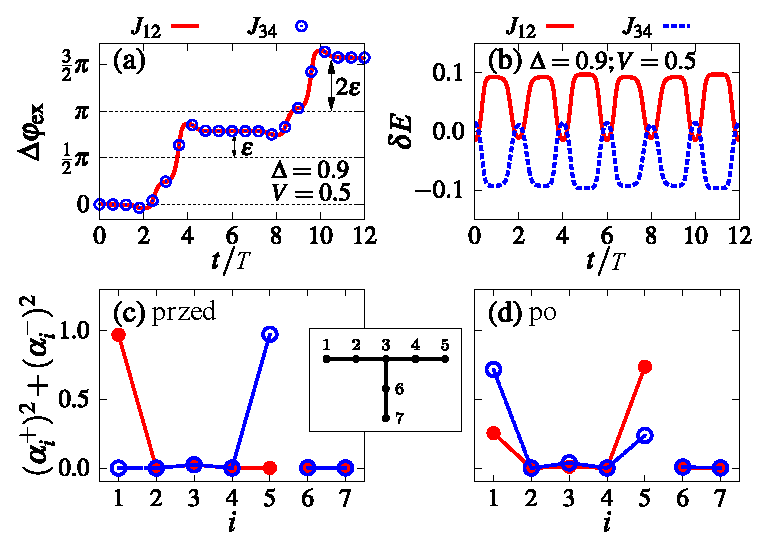
\includegraphics[width=0.8\textwidth]{04-Includes/Figures/PhaseGate/fig4.pdf}
\caption
[Podwójne wyplatanie \textit{MZM} oraz rozkłady przestrzenne przed i po pojedynczym wyplataniu \textit{MZM}.]
{
(a)--(b) Podwójne wyplatanie \MZM.
Wyniki dla $\muuniform=0$, $\muuniform_c=4$ oraz $-4$ odpowiednio dla trójzłącza $\trijunction{12}$ oraz $\trijunction{34}$.
(a) Faza wymiany $\DeltaPhiEx(\timeNormal)$ dla podwójnej operacji wyplatania.
(b) Rozszczepienia energetyczne $\deltaE$ na poszczególnych złączach w czasie ewolucji $\timeNormal/\timePartial$.
(c)--(d) Rozkłady przestrzenne \MZM\ odpowiednio (c)~przed oraz (d)~po pojedynczym protokole wyplatania.
Wyniki dla $\DeltaSCuniform=0.8$, $\Vuniform=0$, $\sites=7$, $\muuniform=0$.
}
\label{fig:phaseGate6}
\end{figure}

Pozostało wyjaśnić ostatni podpunkt~\ref{enum:doubleBraiding} --- podwójne wyplatanie.
Podwójna wymiana \MZM\ będzie odpowiadać działaniu bramki fazowej $\phaseGate$ na stan kwantowy qubitu $\qstate{\psi}=A_0\qstate0+A_1\qstate 1$, gdzie $|A_0|^2$ i $|A_1|^2$ odpowiadają prawdopodobieństwom pomiaru stanu kwantowego odpowiednio w stanie $\qstate 0$ i $\qstate 1$, co do nieistotnej fazy globalnej $\chi$\footnote{Dowód można znaleźć w~dodatku~\ref{chap:derivations}.}
\begin{align}
    \qstate{\psi(2\timeTotal)}  = \eee^{\iu\chi}\phaseGate\qstate{\psi(0)}
    ,\label{eq:qubitPhaseFactorsGained}
\end{align}
gdzie odpowiednio $\chi=\barPhiDyni{e,\,\trijunction{12}}+
     \barPhiDyni{e,\,\trijunction{34}}+
     \barPhiGeoi{e,\,\trijunction{12}} +
    \barPhiGeoi{e,\,\trijunction{34}}$
    to nieistotna część fazy globalnej,
    $\phaseGate=
\begin{bmatrix}
1 & 0 \\
0 & \eee^{\iu\theta}
\end{bmatrix}$ to bramka fazowa.
Faza $\theta$ bramki fazowej wynosi
\begin{equation}
    \theta = -\barDeltaPhiDyni{o,\,\trijunction{12}}-
    \barDeltaPhiDyni{o,\,\trijunction{34}} -
    \barDeltaPhiGeoi{o,\,\trijunction{12}} -
    \barDeltaPhiGeoi{o,\,\trijunction{34}}=-2\pi-4\braidingError\to-4\braidingError.
\end{equation}
Skorzystano tutaj z równania~\labelcref{eq:doubleBraidingGeoPhase,eq:dynPhaseCondition}.
Pominięto również czynnik fazowy $2\pi$, który nie jest istotny do opisu działania bramki fazowej $\phaseGate$, ponieważ istotne znaczenie ma jedynie różnica faz modulo $2\pi$ pomiędzy stanami bazowymi qubitu.

Następnie wykorzystano algorytm opisany w rozdziale~\ref{chap:LIOMs} do generowania struktury przestrzennej \MZM\ na całej ścieżce wyplatania.
Generowano współczynniki $\alphai$ dla każdego chwilowego hamiltonianu $\hatH(\timeNormal)$ dla protokołu pojedynczej wymiany \MZM.
Dla przypomnienia, algorytm polegał na znalezieniu operatorów $\Gammaii_n=\sum_i\alphaii_{ni}\gammai$, dla których relacja komutacji $[\hatH,\Gammaii_n]=0$ była jak \textit{najbardziej} spełniona, w sensie minimalizacji kwadratu normy $\|\Gammaii_n-\barGammaii_n\|^2=0$ [równanie~\eqref{eq:normOpt}].
Operatory będące dowolną kombinacją liniową operatorów spełniających wspomnianą relację komutacji, również spełniają tę relację.
Zakładając, że w układzie mogą znajdować się tylko dwie \MZM: $\Gammaii_1$, $\Gammaii_2$, można rozważyć następujący obrót $\Rotation\omega$ w którym relacja komutacji jest niezmiennicza
\begin{equation}
\vec{\Gammaii}'    = \Rotation \omega \vec{\Gammaii},
\end{equation}
gdzie
\begin{equation}
\vec{\Gammaii}=\begin{bmatrix}
\Gammaii_1\\
\Gammaii_2
\end{bmatrix},\quad
\Rotation\omega=\begin{bmatrix}
\cos\omega & -\sin\omega\\
\sin\omega & \cos\omega
\end{bmatrix}.
\end{equation}
Oczywiste jest, że jeśli operatory $\vec\Gammaii$ komutują z hamiltonianem $[\hatH,\vec\Gammaii]=0$, to  obrócone operatory $\vec\Gammaii'$ również komutują z hamiltonianem $[\hatH,\vec\Gammaii']=0$.
Z tego wynika, że współczynniki $\alphaii_{i1}$, $\alphaii_{i2}$ mogą być zdefiniowane dla dowolnej wartości kąta obrotu $\omega$.
Jako warunek początkowy, dla czasu $\timeNormal=0$, wybrano taki kąt $\omega$, że maksimum współczynników dla $\Gammaii_1$, $\Gammaii_2$
odpowiadało lokalizacji $\Gammaii_1$ na początku lewego drutu, a $\Gammaii_2$ na końcu prawego drutu trójzłącza [patrz rysunek~\ref{fig:phaseGate6}(c)].
Następnie dla każdego kroku ewolucji generowano współczynniki $\alphaii_{in}$ szukając takiego kąta obrotu $\omega(\timeNormal)$, który minimalizował następujący kwadrat odległości operatorów
\begin{equation}
    \| \vec\Gammaii(\timeNormal+\delta\timeNormal)-\vec\Gammaii(\timeNormal)\|^2=\sum_i \sum_n \left[\alphaii_{ni}(\timeNormal+\delta\timeNormal)-\alphaii_{ni}(\timeNormal) \right]^2.
\end{equation}
W przypadku kiedy \MZM\ są ścisłymi całkami ruchu, takie podejście odtwarza standardową wymianę \MZM\ [patrz sekcja~\ref{sec:nonabelianStatistics}]:
\begin{align}
    \Gammaii_1(\timeTotal) = \pm \Gammaii_2(0),\\
    \Gammaii_2(\timeTotal) = \mp \Gammaii_1(0),
\end{align}
co jest równoważne następującemu obrotowi $\vec\Gammaii(\timeTotal) = \Rotation{\pm\frac{\pi}{2}}\vec\Gammaii(0)$.
Jak się okazuje można to uogólnić na przypadek, kiedy \MZM\  przekrywają się podczas wyplatania, gdy pojawia się niezerowy błąd wyplatania $\braidingError$.
Taka ogólna cykliczna ewolucja \MZM\ może zostać zaprezentowana za pomocą następującego równania
\begin{equation}
    \vec\Gammaii(\timeTotal) = \Rotation{\DeltaPhiBerry}\vec\Gammaii(0).
\end{equation}
Po takim wyplataniu dla $\Delta\PhiBerry\neq\pm\frac{\pi}{2}$, nie można  procesu rozumieć jako wymiany \MZM, ponieważ po jego zakończeniu $\Gammaii_1(\timeTotal)$ staje się liniową kombinacją $\Gammaii_1(0)$ oraz $\Gammaii_2(0)$ --- zobacz rysunki~\ref{fig:phaseGate6}(c)--(d). 
To samo dotyczy drugiej \MZM\ $\Gammaii_2(\timeTotal)$.


\ornament

\section{Kalibracja bramki fazowej}





Zestaw uniwersalnych bramek kwantowych nie musi zawierać uniwersalnej bramki fazowej $\phaseGate$ dla dowolnego kąta $\theta$.
Wystarczy, aby ten zbiór zawierał $\phaseGatei{\frac{\pi}{4}}$ dla $\theta=\frac{\pi}{4}$~\cite{nielsen.chuang.2011}.
W~przedstawionej implementacji bramki fazowej na bazie fazy geometrycznej, należałoby skalibrować złącza w taki sposób, aby błąd wyplatania wynosił $\braidingError=\pm\frac{\pi}{16}$.
Błąd wyplatania silnie zależy od rozmiaru układu, co pokazano na rysunku~\ref{fig:phaseGate5}(b).
Na rysunku~\ref{fig:phaseGate7} przedstawiono, jak zależy błąd wyplatania $\braidingError$ od parametrów hamiltonianu ~\eqref{eq:kitaev+braiding}.
Na rysunkach~\ref{fig:phaseGate7}(a)--(b)
przedstawiono zależność $|\braidingError|$ w funkcji oddziaływań $\Vuniform$ oraz parametru nadprzewodnictwa $\DeltaSCuniform$, a
na rysunkach~\ref{fig:phaseGate7}(c)--(d) przedstawiono zależność $|\braidingError|$ w funkcji oddziaływań $\Vuniform$ oraz potencjału $\muuniform$.
Kontrola nad wartością $\DeltaSCuniform$ lub $\Vuniform$ w rzeczywistych eksperymentach może być problematyczna, ale w przypadku kontroli $\muuniform$ taka manipulacja jest wykonalna w prawdziwych realizacjach tego układu.
Za pomocą zmian potencjału chemicznego można kalibrować wartość błędu wyplatania $\braidingError$.

\begin{figure}
\centering
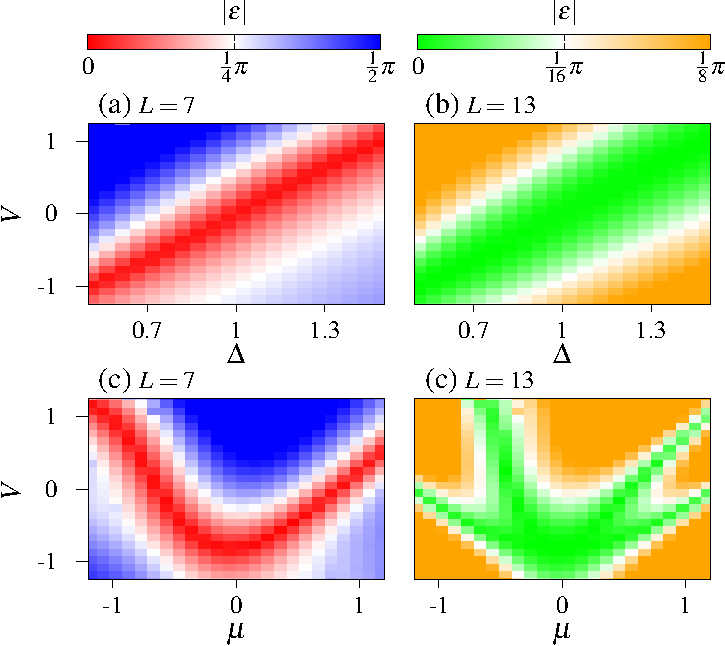
\includegraphics[width=0.75\textwidth]{04-Includes/Figures/PhaseGate/fig5.pdf}
\caption
[Błąd wyplatania w funkcji parametrów hamiltonianu układu.]
{Błąd wyplatania $\braidingError$ (odchylenia fazy $\DeltaPhiBerry$ od $\frac{\pi}2$ w funkcji parametrów hamiltonianu \eqref{eq:kitaev+braiding} układu.
(a)--(b) $\braidingError$ w funkcji $\Vuniform$ oraz $\DeltaSCuniform$ dla $\muuniform=0$ odpowiednio dla $\sites=7$ oraz $13$.
(c)--(d) $\braidingError$ w funkcji $\Vuniform$ oraz $\muuniform$ dla $\DeltaSCuniform=0.6$ odpowiednio dla $\sites=7$ oraz $13$.
}
\label{fig:phaseGate7}
\end{figure}

\begin{figure}
\centering
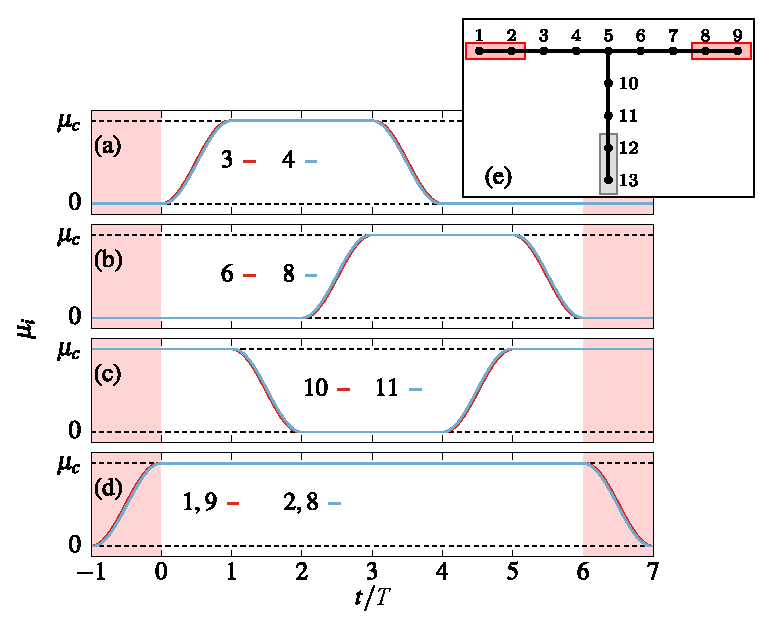
\includegraphics[width=0.8\textwidth]{04-Includes/Figures/PhaseGate/fig10.pdf}
\caption
[Rozszerzony protokół wyplatania.]
{Rozszerzony protokół wyplatania.
Dla czasu $\timeNormal\in[-\timePartial,0]$ \MZM\ są zbliżane do siebie, a dla czasu $\timeNormal\in[6\timePartial,7\timePartial]$ są oddalane na początkowe pozycje.
(a)--(d) Potencjały $\mui$ w funkcji $\timeNormal/\timePartial$ odpowiednio dla
(a) lewego,
(b) prawego,
(c) pionowego łańcucha trójzłącza, które schematycznie zaprezentowano na (e).
(d) Potencjał $\mui(\timeNormal/\timePartial)$ dla węzłów zaznaczonych czerwonym prostokątem na (e).
(e) Numeracja węzłów, szary prostokąt odpowiada \textit{wyłączonym} węzłom, t.j. $\mui(\timeNormal)=\mui_c$.
}
\label{fig:phaseGate8}
\end{figure}


Do tej pory zbadano układ, który nadaje się tylko i wyłącznie do realizacji bramki fazowej.
Przyczyną tego są efekty rozmiarowe --- przekrywanie się \MZM.
To przekrywanie było źródłem błędu wyplatania $\braidingError$, ale równocześnie dla przypadku przekrywania się \MZM,
 nie mamy gwarancji ochrony topologicznej i nie możemy zrealizować w \textit{bezpieczny} sposób wszystkich operacji z grupy warkoczowej $\braidGroup$.
W celu zagwarantowania ochrony topologicznej, \MZM\ powinny być odseparowane przestrzennie jak to tylko możliwe ($\sites\to\infty$).
Kiedy ten warunek jest spełniony, podwójna wymiana \MZM, należących do tego samego trójzłącza odpowiada operacji bramki $\zgate$ [patrz rysunek~\ref{fig:phaseGate2}(a)].
W celu realizacji bramki fazowej opisanej w poprzedniej sekcji, najpierw należałoby zbliżyć do siebie \MZM\ na skończoną odległość na obu trójzłączach $\trijunction{12}$, $\trijunction{34}$ (równocześnie muszą być spełnione wszystkie warunki wspomniane w~pkt. \labelcref{enum:oddSites,enum:negativePotential,enum:doubleBraiding} w sekcji~\ref{sec:phaseGateRealization}).
Zasadę działania bramki fazowej schematycznie przedstawiono na rysunku~\ref{fig:phaseGate2}(b).
W celu symulacji bramki fazowej zmodyfikowano potencjał $\mui(\timeNormal)$ tak, aby w czasie ewolucji uwzględniony był proces zbliżania i oddalania \MZM.
Nowy zmodyfikowany potencjał przedstawiono na rysunku~\ref{fig:phaseGate8}.
Zacieniowanym obszarem na wykresie zaznaczono odpowiednio proces zbliżania \MZM\ ($\timeNormal\in[-\timePartial,0]$) oraz oddalania ($\timeNormal\in[6\timePartial,7\timePartial]$).
Po zbliżeniu \MZM, odbywał się proces wyplatania dla trójzłącza o ograniczonej wielkości $\sites'$.
Stosowana metoda numeryczna ogranicza nas do wielkości badanych układów $\sites$.
W tym celu do zbadania rozszerzonego protokołu wykorzystaliśmy skalowanie rozmiarowe \acrshort{FSS}.
Na rysunku~\ref{fig:phaseGate9} przedstawiono, w jaki sposób dokonywano skalowania rozmiarowego układu $\sites$, równocześnie nie zmieniając odległości na jaką zbliżamy \MZM --- rozmiar ograniczonego złącza $\sites'$.



\begin{figure}
\centering
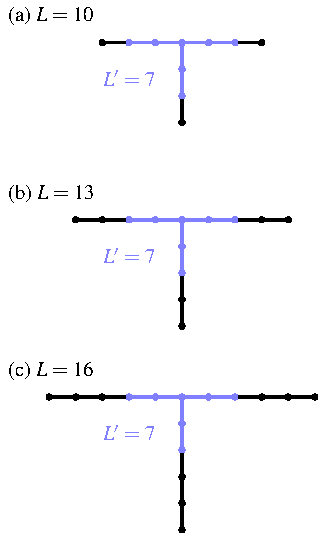
\includegraphics[width=0.4\textwidth]{04-Includes/Figures/PhaseGate/fig7.pdf}
\caption
[Skalowanie rozmiarowe trójzłącza dla rozszerzonego protokołu wyplatania.]
{Skalowanie rozmiarowe trójzłącza dla rozszerzonego protokołu wyplatania.
Niebieskim kolorem zaznaczono węzły należące do trójzłącza ograniczonego -- po zbliżeniu \MZM.
Początkowo \MZM\ znajdują się na krańcach całego złącza, następnie są zbliżane do ograniczonego złącza, wyplatane i przemieszczane na początkowe pozycje.
}
\label{fig:phaseGate9}
\end{figure}


\begin{figure}
\centering
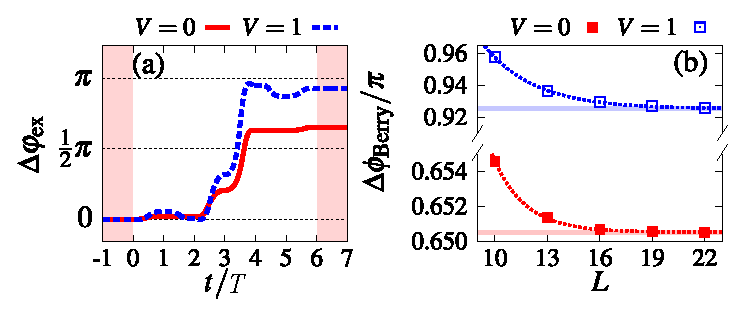
\includegraphics[width=0.8\textwidth]{04-Includes/Figures/PhaseGate/fig6.pdf}
\caption
[Faza wymiany oraz faza geometryczna dla rozszerzonego protokołu wyplatania \textit{MZM}.]
{
Wyplatanie \MZM, które są zbliżane $\timeNormal\in[-\timePartial,0]$ oraz oddalane $\timeNormal\in[6\timePartial,7\timePartial]$.
Wyniki dla $\Delta=0.8$, $\muuniform=0$, $\sites'=7$.
(a) Faza wymiany $\DeltaPhiEx$ dla $\sites=19$.
(b) Skalowanie rozmiarowe fazy geometrycznej $\DeltaPhiBerry$.
Poziome (ciągłe) linie odpowiadają ekstrapolowanym wartościom $\DeltaPhiBerry(\infty)$ dla poszczególnych przypadków.
Do dopasowania wykorzystano funkcję $\DeltaPhiBerry(\sites)=a\exp(-b\sites)+\DeltaPhiBerry(\infty)$ (zaznaczono linią przerywaną).
}
\label{fig:phaseGate10}
\end{figure}


Na rysunku~\ref{fig:phaseGate10}(a) przedstawiono fazę wymiany $\DeltaPhiEx(\timeNormal)$ dla układu o całkowitym rozmiarze złącza $\sites=19$ i ograniczonego złącza $\sites'=7$.
Analogicznie jak na rysunku~\ref{fig:phaseGate8}, na rysunku~\ref{fig:phaseGate10}(a) cieniowanym obszarem zaznaczono czas dla którego następował proces zbliżania/oddalania \MZM.
Zmiany fazy podczas zbliżania/oddalania, są bardzo małe, ale nie pomijalne.
Przedstawiona implementacja bramki fazowej w sekcji~\ref{sec:phaseGateRealization} bazuje na błędzie wyplatania, $\braidingError$, który powinien mieć skończoną, niezerową wartość również w granicy termodynamicznej $\sites\to\infty$, tak długo jak $\sites'\ll\infty$.
W najlepszym, pożądanym przypadku $\braidingError$ powinien silnie zależeć od odległości na jaką zbliżamy \MZM, czyli na rozmiar ograniczonego złącza $\sites'$.
Natomiast, $\braidingError$ powinien słabo zależeć od $\sites$.
W celu badania w jaki sposób  $\braidingError$ zależy od rozmiaru układu, ustalono $\sites'=7$ na stałe i zmieniano rozmiar układu $\sites$ zgodnie z rysunkiem~\ref{fig:phaseGate9}.
Na rysunku~\ref{fig:phaseGate10}(b) przedstawiono skalowanie rozmiarowe otrzymanej fazy Berry'ego~$\DeltaPhiBerry$ po zbliżaniu, wyplataniu i oddalaniu \MZM.
W odróżnieniu od przedstawionych wyników na rysunku~\ref{fig:phaseGate5}(b), wyniki przedstawione na rysunku~\ref{fig:phaseGate10} pokazują, że w takim wypadku błąd wyplatania nie jest efektem rozmiarowym.
Wydaje się, że nawet w granicy termodynamicznej $\sites\to\infty$, wartość błędu wyplatania jest $\braidingError\neq0$, o ile $\sites'$ jest skończone i \MZM\ przekrywają się podczas procedury wyplatania.
Słaba zależność $\DeltaPhiBerry$ od rozmiaru układu $\sites$ przedstawiona na rysunku~\ref{fig:phaseGate10}(b) może być związana z tzw. \textit{wyciekiem} \MZM\ do obszaru trójzłącza trywialnego~\cite{klinovaja.loss.2012,ruiz-tijerina.vernek.2015,ptok.kobialka.2017}.

\ornament

\section*{Podsumowanie}

Przedstawiono minimalny zestaw bramek dla  realizacji qubitu bazującego na \MZM.
Na rysunku~\ref{fig:phaseGate2}(a) oraz ~\ref{fig:phaseGate2}(c) 
przedstawiono schematycznie implementację topologiczne chronionych bramek, odpowiednio $\zgate$ oraz $\xgate$~\cite{alicea.oreg.2011,bravyi.2006}.
W obu przypadkach zakłada się, że \MZM\ nie przekrywają się podczas całej ewolucji.
Na rysunku~\ref{fig:phaseGate2}(b) przedstawiono protokół bramki fazowej $\phaseGate$ zrealizowanej przez wyplatanie przekrywających się \MZM.
Wspomniana bramka fazowa zależy od fazy geometrycznej, a nie od, jak w przypadku standardowej realizacji, fazy dynamicznej~\cite{sarma.freedman.2015}.
Opisany protokół bramki fazowej wymaga przekrywających się \MZM.
Przekrywające się \MZM\ nie są \textit{stricte} całkami ruchu.
W takim wypadku, podczas wyplatania qubit nabiera odpowiednio fazy dynamicznej oraz geometrycznej.
Przedstawiony protokół w naszej pracy~\cite{wieckowski.mierzejewski.2020} gwarantuje eliminację wspomnianej fazy dynamicznej i~równocześnie powoduje, że przesunięcie fazowe tak skonstruowanej bramki fazowej zależy tylko i~wyłącznie od fazy geometrycznej.
Faza dynamiczna może zostać wyeliminowana, kiedy dwa identyczne trójzłącza reprezentujące pojedynczy qubit, opisane są przez hamiltonian z symetrią cząstka--dziura i posiadają nieparzystą liczbę węzłów sieci.
Jedyna różnica w~tym protokole od topologicznie chronionych operacji polega na zbliżeniu do siebie \MZM\ na skończoną odległość przed procedurą wyplatania.
Takie zbliżenie ma zapewnić zniesienie degeneracji na skutek przekrywania się \MZM.
Po zakończonym wyplataniu, \MZM\ rozsuwane są na początkową, \textit{bezpieczną}, odległość, w której możliwe są operacje z zagwarantowaną ochroną topologiczną.
Błąd opisanej bramki fazowej na bazie fazy geometrycznej powinien być mniejszy od standardowej bramki fazowej, której przesunięcie fazowe zależy od fazy dynamicznej, ponieważ faza geometryczna nie zależy jawnie od czasu.
Nie zmienia to oczywiście faktu, że realizacja takiej bramki fazowej bazującej na fazie geometrycznej powinna zostać uzupełniona o odpowiednie korekty błędów.

\ornament
